\ifx\wholebook\relax \else
% ------------------------

\documentclass[b5paper]{article}
\usepackage[nomarginpar
  %, margin=.5in
]{geometry}

\addtolength{\oddsidemargin}{-0.05in}
\addtolength{\evensidemargin}{-0.05in}
\addtolength{\textwidth}{0.1in}

\usepackage[en]{../../../prelude}

\setcounter{page}{1}

\begin{document}

\title{Red-black tree}

\author{Xinyu LIU
\thanks{{\bfseries Xinyu LIU} \newline
  Email: liuxinyu95@gmail.com \newline}
  }

\maketitle
\fi

\markboth{Red-black tree}{Elementary Algorithms}

\ifx\wholebook\relax
\chapter{Red-black tree}
\numberwithin{Exercise}{chapter}
\fi

\section{Introduction}
\label{sec:rbtree-introduction} \index{red-black tree}

In chapter 2, there is an example about binary search tree. We use it as a dictionary to count the word occurrence in a text. One may want to feed a address book to a binary search tree, and use it to look up the contact as below example program:

\lstset{frame = single}
\begin{lstlisting}[language=Bourbaki]
void addrBook(Input in) {
    bst<string, string> dict
    while (string name, string addr) = read(in)) {
        dict[name] = addr
    }
    loop {
        string name = read(console)
        var addr = dict[name]
        if (addr == null) {
            print("not found")
        } else {
            print("address is", addr)
        }
    }
}
\end{lstlisting}

Unlike the word counter program, this one performs poorly, especially when search names like Zara, Zed, Zulu, etc. This is because the address entries are typically listed in lexicographic order, i.e. the names are input in ascending order. If insert numbers 1, 2, 3, ..., $n$ to a binary search tree, it ends up like in figure \ref{fig:unbalanced-tree}. It is an extremely unbalanced binary search tree. The $lookup()$ is bound to $O(h)$ time for a tree with height $h$. When the tree is well balanced, the performance is $O(\lg n)$, where $n$ is the number of elements in the tree. But in this extreme case, the performance downgrades to $O(n)$. It is not better than list scan.

\begin{figure}[htbp]
  \centering
  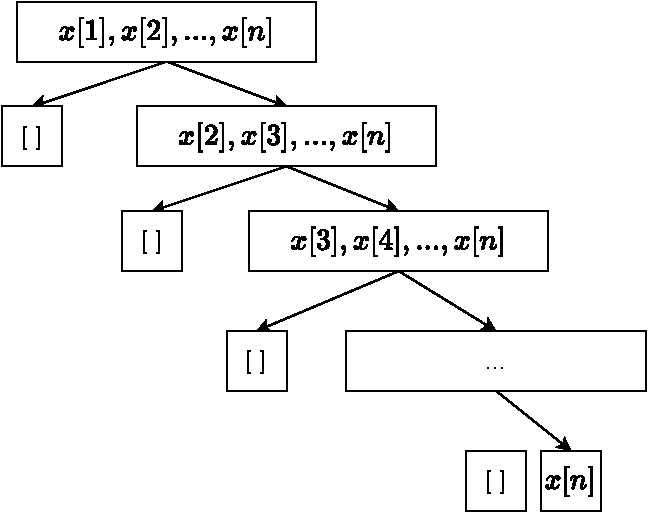
\includegraphics[scale=0.5]{img/unbalanced.ps}
  \caption{unbalanced tree}
  \label{fig:unbalanced-tree}
\end{figure}

\begin{Exercise}
\Question{For a big address entry list in lexicographic order, one may want to speed up the address book building with two concurrent tasks. One reads from the head, while the other reads from the tail. Till they meet at some middle point. What does the binary search tree look like? What if split the list into multiple sections to scale the concurrency?}
\Question{Find more cases to exploit a binary search tree, for example in figure \ref{fig:unbalanced-trees}.}
\end{Exercise}

\begin{figure}[htbp]
  \centering
  \subcaptionbox{}{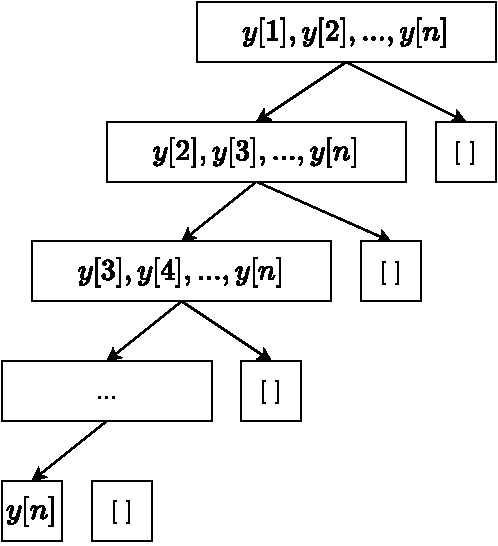
\includegraphics[scale=0.4]{img/unbalanced-2.ps}}
  \subcaptionbox{}{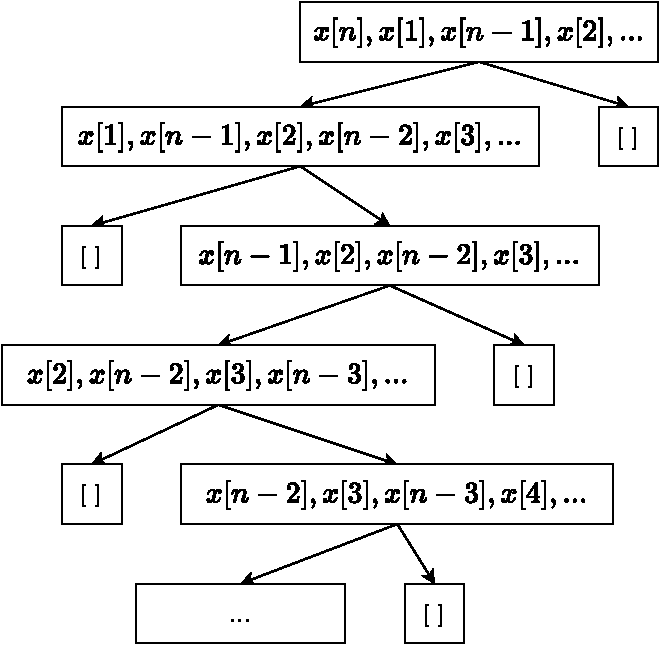
\includegraphics[scale=0.4]{img/unbalanced-zigzag.ps}} \\
  \subcaptionbox{}{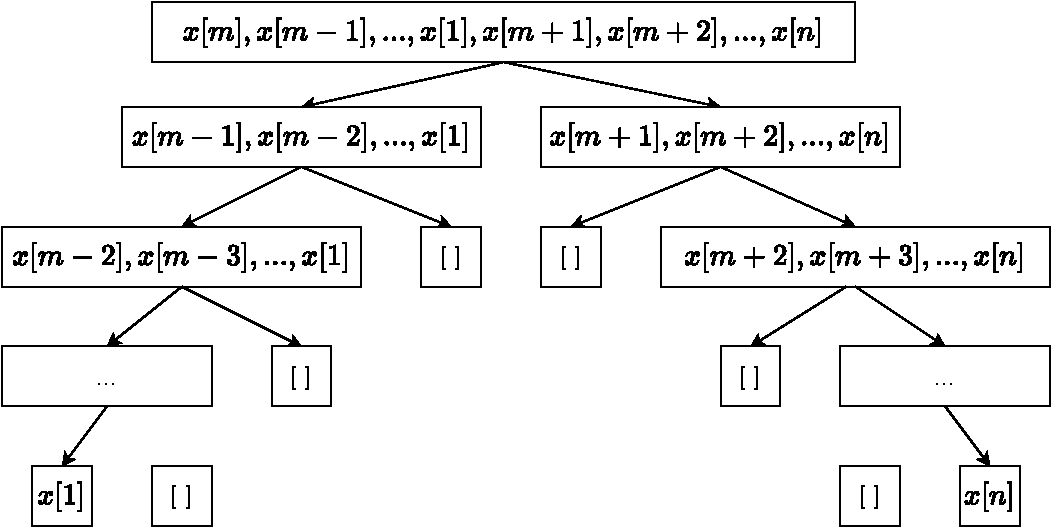
\includegraphics[scale=0.4]{img/unbalanced-3.ps}}
  \caption{Unbalanced trees}
  \label{fig:unbalanced-trees}
\end{figure}

\subsection{Balance}
To avoid extremely unbalanced case, we can shuffle the input(12.4 in \cite{CLRS}), however, there is situation that the input is fed from user, that we can not randomize the sequence. People developed solutions to make the tree balanced. They mostly rely on the rotation operation. Rotation changes the tree structure while maintain the elements ordering. This chapter introduces the red-black tree, the widely used self-adjusting balanced binary search tree. Next chapter is about AVL tree, another self-balanced tree. Chapter 8 introduce the splay tree, which adjust the tree in steps to make it balanced.

\subsection{Tree rotation}
\index{tree rotation}

\begin{figure}[htbp]
   \centering
   \setlength{\unitlength}{1cm}
   \begin{picture}(10, 4)
   \put(5, 2){$\Longleftrightarrow$}
   \subcaptionbox{}{\includegraphics[scale=0.4]{img/rotate-r.ps}}
   \subcaptionbox{}{\includegraphics[scale=0.4]{img/rotate-l.ps}}
   \end{picture}
   \\
   \begin{picture}(1, 0.5)\end{picture} %pad
   \caption{`left rotate' transforms the tree from left to right; `right rotate' is inverse.}
   \label{fig:tree-rotation}
\end{figure}

Tree rotation transforms the tree structure while keeping the in-order traverse result unchanged. There are multiple binary search trees generate the same ordered element sequence. Figure \ref{fig:tree-rotation} shows the tree rotation.

Tree rotation can be defined with pattern matching:

\be
\begin{array}{rcl}
rotate_l\ ((a, X, b), Y, c) & = & (a, X, (b, Y, c)) \\
rotate_l\ T & = & T \\
\end{array}
\ee

and

\be
\begin{array}{rcl}
rotate_r\ (a, X, (b, Y, c)) & = & ((a, X, b), Y, c)) \\
rotate_r\ T & = & T \\
\end{array}
\ee

We can also implement tree rotation imperatively. We need re-assign children and parent node references. When rotate, we pass both tree root $T$, and the node $x$ to apply rotation:

\begin{algorithmic}[1]
\Function{Left-Rotate}{$T, x$}
  \State $p \gets$ \Call{Parent}{$x$}
  \State $y \gets$ \Call{Right}{$x$} \Comment{assume $y \ne$ NIL}
  \State $a \gets$ \Call{Left}{$x$}
  \State $b \gets$ \Call{Left}{$y$}
  \State $c \gets$ \Call{Right}{$y$}
  \State \Call{Replace}{$x, y$}  \Comment{replace node $x$ with $y$}
  \State \Call{Set-Subtrees}{$x, a, b$} \Comment{Set $a, b$ as the sub-trees of $x$}
  \State \Call{Set-Subtrees}{$y, x, c$} \Comment{Set $x, c$ as the sub-trees of $y$}
  \If{$p = $ NIL}  \Comment{$x$ is the previous root}
    \State $T \gets y$
  \EndIf
  \State \Return $T$
\EndFunction
\end{algorithmic}

The \textproc{Right-Rotate} is symmetric, we leave it as exercise. The procedure \textproc{Replace}($x$, $y$) uses node $y$ to replace $x$:

\begin{algorithmic}[1]
\Function{Replace}{$x, y$}
  \State $p \gets$ \Call{Parent}{$x$}
  \If{$p$ = NIL} \Comment{$x$ is the root}
    \If{$y \ne$ NIL}
           \Call{Parent}{$y$} $\gets$ NIL
    \EndIf
  \ElsIf{\Call{Left}{$p$} $= x$}
    \State \Call{Set-Left}{$p$, $y$}
  \Else
    \State \Call{Set-Right}{$p$, $y$}
  \EndIf
  \State \Call{Parent}{$x$} $\gets$ NIL
\EndFunction
\end{algorithmic}

Procedure \textproc{Set-Subtrees}($x, L, R$) assigns $L$ as the left sub-tree of $x$, and $R$ as the right sub-tree.

\begin{algorithmic}[1]
\Function{Set-Children}{$x, L, R$}
  \State \Call{Set-Left}{$x, L$}
  \State \Call{Set-Right}{$x, R$}
\EndFunction
\end{algorithmic}

It further calls \textproc{Set-Left} and \textproc{Set-Right} to set the two sub-trees:

\begin{algorithmic}[1]
\Function{Set-Left}{$x, y$}
  \State \Call{Left}{$x$} $\gets y$
  \If{$y \ne$ NIL}
    \Call{Parent}{$y$} $\gets x$
  \EndIf
\EndFunction

\Statex

\Function{Set-Right}{$x, y$}
  \State \Call{Right}{$x$} $\gets y$
  \If{$y \ne$ NIL}
    \Call{Parent}{$y$} $\gets x$
  \EndIf
\EndFunction
\end{algorithmic}

We can see how pattern matching simplifies the tree rotation. Based on this idea, Okasaki developed the purely functional algorithm for red-black tree\cite{okasaki}.

\begin{Exercise}
\Question{Implement the \textproc{Right-Rotate} algorithm.}
\end{Exercise}

\section{Definition}
\index{red-black tree}

A red-black tree is a self-balancing binary search tree\cite{wiki-rbt}. It is essentially equivalent to 2-3-4 tree\footnote{Chapter 7 B-trees. For any 2-3-4 tree, there is at least one red-black tree has the same ordered data.}. By coloring the node red or black, and perform rotation, red-black tree provides a efficient way to keep the tree balanced. On top of the binary search tree definition, we label the node with a color. We say it is a red-black tree if the coloring satisfies the following 5 rules(\cite{CLRS} pp273):

\index{red-black tree!red-black properties}
\begin{enumerate}
\item Every node is either red or black.
\item The root is black.
\item Every leaf (NIL) is black.
\item If a node is red, then both sub-trees are black.
\item For each node, all paths from the node to descendant leaves contain the same number of black nodes.
\end{enumerate}

Why do they keep the red-black tree balanced? The key point is that, the longest path from root to leaf can not be as 2 times longer than the shortest path. Consider rule 4, there are not any two adjacent red nodes. Therefore, the shortest path contains only black nodes. Any longer path must have red one. In addition, rule 5 ensures all paths have the same number of black nodes. It eventually ensures any path is not 2 times longer than others\cite{wiki-rbt}. Figure \ref{fig:rbt-example-with-nil} gives an example red-black tree.

\begin{figure}[htbp]
  \centering
  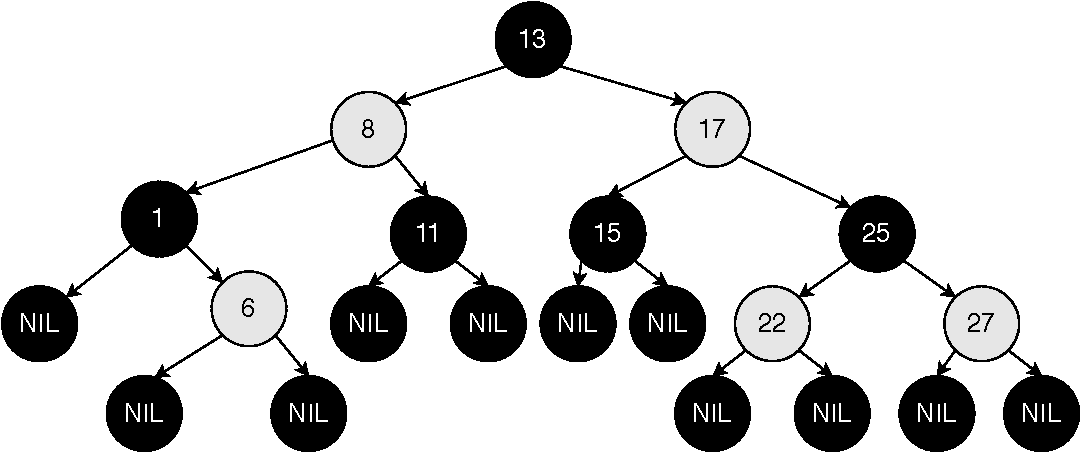
\includegraphics[scale=0.6]{img/rbt-example-with-nil.ps}
  \caption{A red-black tree}
  \label{fig:rbt-example-with-nil}
\end{figure}

As all NIL nodes are black, we can hide them in the figure, as shown in figure \ref{fig:rbt-example}. All operations including $lookup$, $min/max$, are same as the binary search tree. However, the $insert$ and $delete$ are special, as we need maintain the coloring rules.

\begin{figure}[htbp]
  \centering
  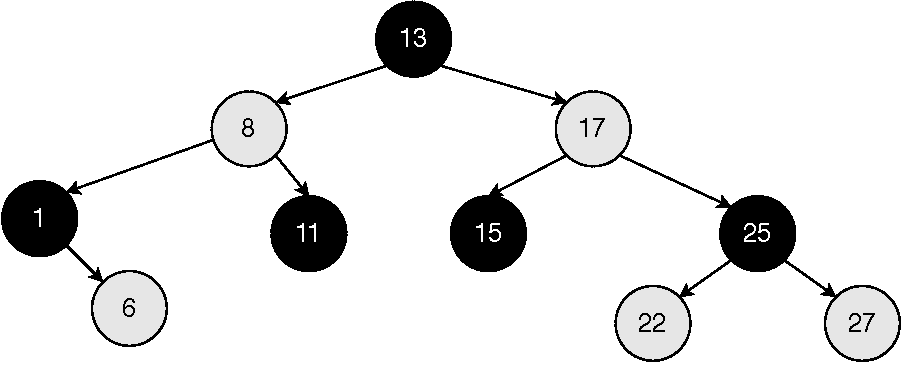
\includegraphics[scale=0.6]{img/rbt-example.ps}
  \caption{Hide the NIL nodes}
  \label{fig:rbt-example}
\end{figure}

Below example program adds the color field atop binary search tree definition:

\begin{Haskell}
data Color = R | B
data RBTree a = Empty
              | Node Color (RBTree a) a (RBTree a)
\end{Haskell}

\begin{Exercise}
\Question{Prove the height $h$ of a red-black tree of $n$ nodes is at most $2 \lg (n+1)$}
\end{Exercise}

\section{Insert}
\index{red-black tree!insert}

The idea of red-black tree $insert$ algorithm contains two steps. The first step is same as the binary search tree insertion. After that the tree may becomes unbalanced, we then fix it to resume the red-black tree coloring conditions in the second step. When insert a new element, we always make it a red node. Unless the new node is the root, we won't break any coloring rules except for the 4-th. This is because it may bring two adjacent red nodes. Okasaki finds there are 4 cases violate rule 4. All have two adjacent red nodes. They share a uniformed structure after fixing\cite{okasaki} as shown in figure \ref{fig:insert-fix}.

\begin{figure}[htbp]
  \centering
  \setlength{\unitlength}{1cm}
  \begin{picture}(15, 15)
    % arrows
    \put(4.5, 9.5){\vector(1, -1){1}}
    \put(4.5, 5){\vector(1, 1){1}}
    \put(10, 9.5){\vector(-1, -1){1}}
    \put(10, 5){\vector(-1, 1){1}}
    % graphics
    \put(0, 7){\includegraphics[scale=0.5]{img/insert-ll.ps}}
    \put(0, 0){\includegraphics[scale=0.5]{img/insert-lr.ps}}
    \put(7, 7){\includegraphics[scale=0.5]{img/insert-rr.ps}}
    \put(8.5, 0){\includegraphics[scale=0.5]{img/insert-rl.ps}}
    \put(2, 5){\includegraphics[scale=0.5]{img/insert-fixed.ps}}
  \end{picture}
  \caption{Fix 4 cases to the same structure in the center.}
  \label{fig:insert-fix}
\end{figure}

All 4 transformations move the redness one level up. When perform bottom-up recursive fixing, the last step will re-color the root as red. While rule 2 requires the root always be black. We need revert the root back to black finally. By using pattern matching, we can define a $balance$ function to fix the red-black tree. Denote the color as $\mathcal{C}$ with values black $\mathcal{B}$, and red $\mathcal{R}$. A none empty node is present as $T = (\mathcal{C}, l, k, r)$.

\be
\begin{array}{rcl}
%\text{up left:} & & \\
balance\ \mathcal{B}\ (\mathcal{R}, (\mathcal{R}, a, x, b), y, c)\ z\ d & = & (\mathcal{R}, (\mathcal{B}, a, x, b), y, (\mathcal{B}, c, z, d)) \\
%\text{up right:} & & \\
balance\ \mathcal{B}, (\mathcal{R}, a, x, (\mathcal{R}, b, y, c))\ z\ d  & = & (\mathcal{R}, (\mathcal{B}, a, x, b), y, (\mathcal{B}, c, z, d)) \\
%\text{bottom left:} & & \\
balance\ \mathcal{B}\ a\ x\ (\mathcal{R}, b, y, (\mathcal{R}, c, z, d)) & = & (\mathcal{R}, (\mathcal{B}, a, x, b), y, (\mathcal{B}, c, z, d))  \\
%\text{bottom right:} & & \\
balance\ \mathcal{B}\ a\ x\ (\mathcal{R}, (\mathcal{R}, b, y, c), z, d) & = & (\mathcal{R}, (\mathcal{B}, a, x, b), y, (\mathcal{B}, c, z, d))  \\
%\text{otherwise:} & & \\
balance\ T & = & T \\
\end{array}
\ee

Where the last clause says if the tree is not in any 4 patterns, then we leave it unchanged. With $balance$ defined, we can modify the binary search tree $insert$ algorithm for red-black tree:

\be
insert\ T\ k = makeBlack\ (ins\ T\ k)
\ee

where

\be
\begin{array}{rcl}
ins\ \nil\ k & = & (\mathcal{R}, \nil, k, \nil) \\
ins\ (\mathcal{C}, l, k', r)\ k & = & \begin{cases}
  k < k': & balance\ \mathcal{C}\ (ins\ l\ k)\ k'\ r \\
  k > k': & balance\ \mathcal{C}\ l\ k'\ (ins\ r\ k) \\
  \end{cases}
\end{array}
\ee

If the tree is empty, we create a red leaf of $k$; otherwise, let the sub-trees and the key be $l$, $r$, $k'$, we compare $k$ and $k'$, then recursively insert $k$ to a sub-tree. After that, we call $balance$ to fix the coloring, then force the root to be black finally.

\be
makeBlack\ (\mathcal{C}, l, k, r) = (\mathcal{B}, l, k, r)
\ee

Below is the corresponding example program:

\begin{Haskell}
insert t x = makeBlack $ ins t where
    ins Empty = Node R Empty x Empty
    ins (Node color l k r)
        | x < k     = balance color (ins l) k r
        | otherwise = balance color l k (ins r)
    makeBlack(Node _ l k r) = Node B l k r

balance B (Node R (Node R a x b) y c) z d =
                Node R (Node B a x b) y (Node B c z d)
balance B (Node R a x (Node R b y c)) z d =
                Node R (Node B a x b) y (Node B c z d)
balance B a x (Node R b y (Node R c z d)) =
                Node R (Node B a x b) y (Node B c z d)
balance B a x (Node R (Node R b y c) z d) =
                Node R (Node B a x b) y (Node B c z d)
balance color l k r = Node color l k r
\end{Haskell} %$

We skip to handle the duplicated keys. If the key to be inserted already exists, we can overwrite it or drop the duplicated one (\cite{CLRS}, pp269). Figure \ref{fig:insert-example} shows two red-black trees built from sequence 11, 2, 14, 1, 7, 15, 5, 8, 4 and 1, 2, ..., 8. The second example demonstrates the tree is well balanced even for ordered input.

\begin{figure}[htbp]
  \centering
  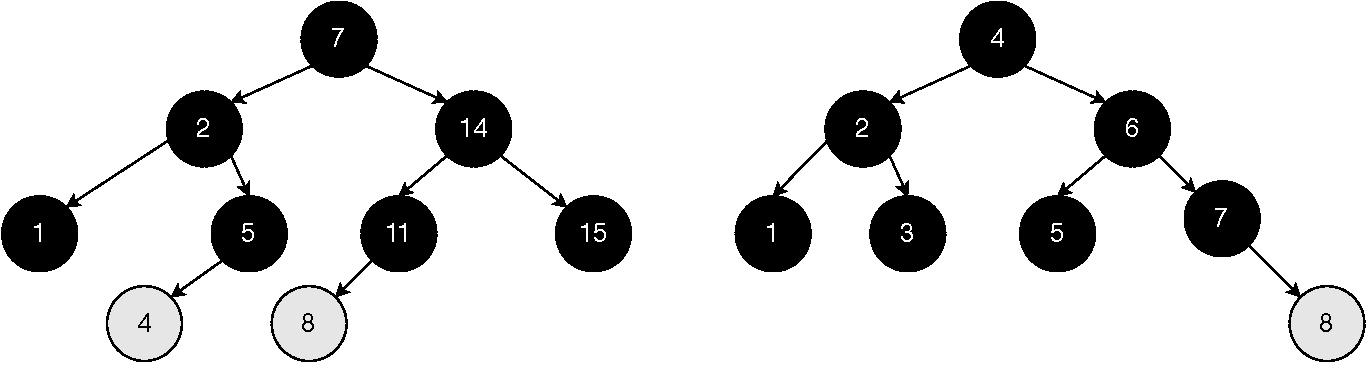
\includegraphics[scale=0.5]{img/insert-haskell.ps}
  \caption{Red-black tree examples}
  \label{fig:insert-example}
\end{figure}

The algorithm performs top-down recursive insertion and fixing. It is bound to $O(h)$ time, where $h$ is the height of the tree. As the red-black tree coloring rules are maintained, $h$ is the logarithm to the number of nodes $n$. The overall performance is $O(\lg n)$.

\begin{Exercise}
\Question{Implement the $insert$ algorithm without using pattern matching, but test the 4 cases separately.}
\end{Exercise}

\section{Delete}
\index{red-black tree!delete}

Delete is more complex than insert. Sometimes, we only need build the read-only tree, then offer it for frequently looking up\cite{okasaki-blog}. We'll show that it's possible to implement red-black tree $delete$ algorithm in purely functional way\footnote{Actually, the tree is rebuilt, although the common part is reused. This feature is called `persist'}. There are alternatives to mimic delete. For example, mark the deleted node with a flag, and later rebuild the tree when the number of deleted nodes exceeds 50\%. Delete may also violate the red-black tree coloring rules. We use the same idea to apply fixing after binary search tree delete. The coloring violation only happens when delete a black node, according to rule 5. The black nodes along the path decreases by one, hence not all paths contain the same number of black nodes.

To resume the blackness, we introduce a special `doubly-black' node(\cite{CLRS}, pp290). One such node is counted as 2 black nodes. When delete a black node $x$, we can move the blackness either up to its parent node or down to one sub-tree. Let this node be $y$ that accepts the blackness. If $y$ was red, we turn it black; if $y$ was already black, we make it `doubly-black', denoted as $\mathcal{B}^2$. Below example program adds the `doubly-black' support:

\begin{Haskell}
data Color = R | B | BB
data RBTree a = Empty | BBEmpty
              | Node Color (RBTree a) a (RBTree a)
\end{Haskell}

Because the empty leaves are all black, when push the blackness down to a leaf, it become `doubly-black' empty (\texttt{BBEmpty}). We also denote it as $\pmb{\varnothing}$. The first step to delete a node is to perform the normal binary search tree delete; then next, if the sliced out node is black, we move the blackness, and fix the red-black tree coloring.

\be
delete = makeBlack \circ del
\ee

This is in Curried form. When delete the only element from the tree, it becomes empty. To cover this case, we modify $makeBlack$ as below:

\be
\begin{array}{rcl}
makeBlack\ \nil & = & \nil \\
makeBlack\ (\mathcal{C}, l, k, r) & = & (\mathcal{B}, l, k, r) \\
\end{array}
\ee

Where $del$ accepts the tree and the element $k$ to be delete:

\be
\begin{array}{rcl}
del\ \nil\ k & = & \nil \\
del\ (\mathcal{C}, l, k', r)\ k & = & \begin{cases}
  k < k': & fixB^2(\mathcal{C}, (del\ l\ k), k', r) \\
  k > k': & fixB^2(\mathcal{C}, l, k', (del\ r\ k)) \\
  k = k': & \begin{cases}
    l = \nil: & (\mathcal{C} = \mathcal{B} \mapsto shiftB\ r, r) \\
    r = \nil: & (\mathcal{C} = \mathcal{B} \mapsto shiftB\ l, l) \\
    else: & fixB^2(\mathcal{C}, l, k'', (del\ r\ k'')) \\
    & \text{where}\ k'' = min(r) \\
  \end{cases}
\end{cases}
\end{array}
\ee

When the tree is empty, the result is $\nil$; otherwise, we compare the key $k'$ in the tree with $k$. If $k < k'$, we recursively
delete $k$ from the left sub-tree; if $k > k'$ then delete from the right. Because the recursive result may contain doubly-black node, we need apply $fixB^2$ to fix it. When $k = k'$, we need splice it out. If either sub-tree is empty, we replace it with the other sub-tree, then shift the blackness if the spliced node is black. This is represented with McCarthy form $(p \mapsto a, b)$, which is equivalent to `(if $p$ then $a$ else $b$)'. If neither sub-tree is empty, we cut the minimum element $k'' = min(r)$, and use $k''$ to replace $k$.

To reserve the blackness, $shiftBlack$ makes a black node doubly-black, and forces it black for all other cases (it flips doubly-black to normal black when applied twice). Below is the example program (except the doubly-black fixing part).

\begin{Haskell}
delete :: (Ord a) => RBTree a -> a -> RBTree a
delete t k = makeBlack $ del t k where
    del Empty _ = Empty
    del (Node color l k' r) k
        | k < k' = fixDB color (del l k) k' r
        | k > k' = fixDB color l k' (del r k)
        | isEmpty l = if color == B then shiftBlack r else r
        | isEmpty r = if color == B then shiftBlack l else l
        | otherwise = fixDB color l k'' (del r k'') where k''= min r
    makeBlack (Node _ l k r) = Node B l k r
    makeBlack _ = Empty

shiftBlack (Node B l k r) = Node BB l k r
shiftBlack (Node _ l k r) = Node B  l k r
shiftBlack Empty = BBEmpty
shiftBlack BBEmpty = Empty
\end{Haskell}

The $fixB^2$ function eliminates the doubly-black node by rotation and re-coloring. The doubly-black node can be branch node or empty $\pmb{\varnothing}$. There are three cases:

\textbf{Case 1}. {\em The sibling of the doubly-black node is black, and it has a red sub-tree.} We can fix this case with a rotation. There are 4 sub-cases, all can be transformed to a uniformed pattern, as shown in figure \ref{fig:del-case1}.

\begin{figure}[htbp]
  \centering
  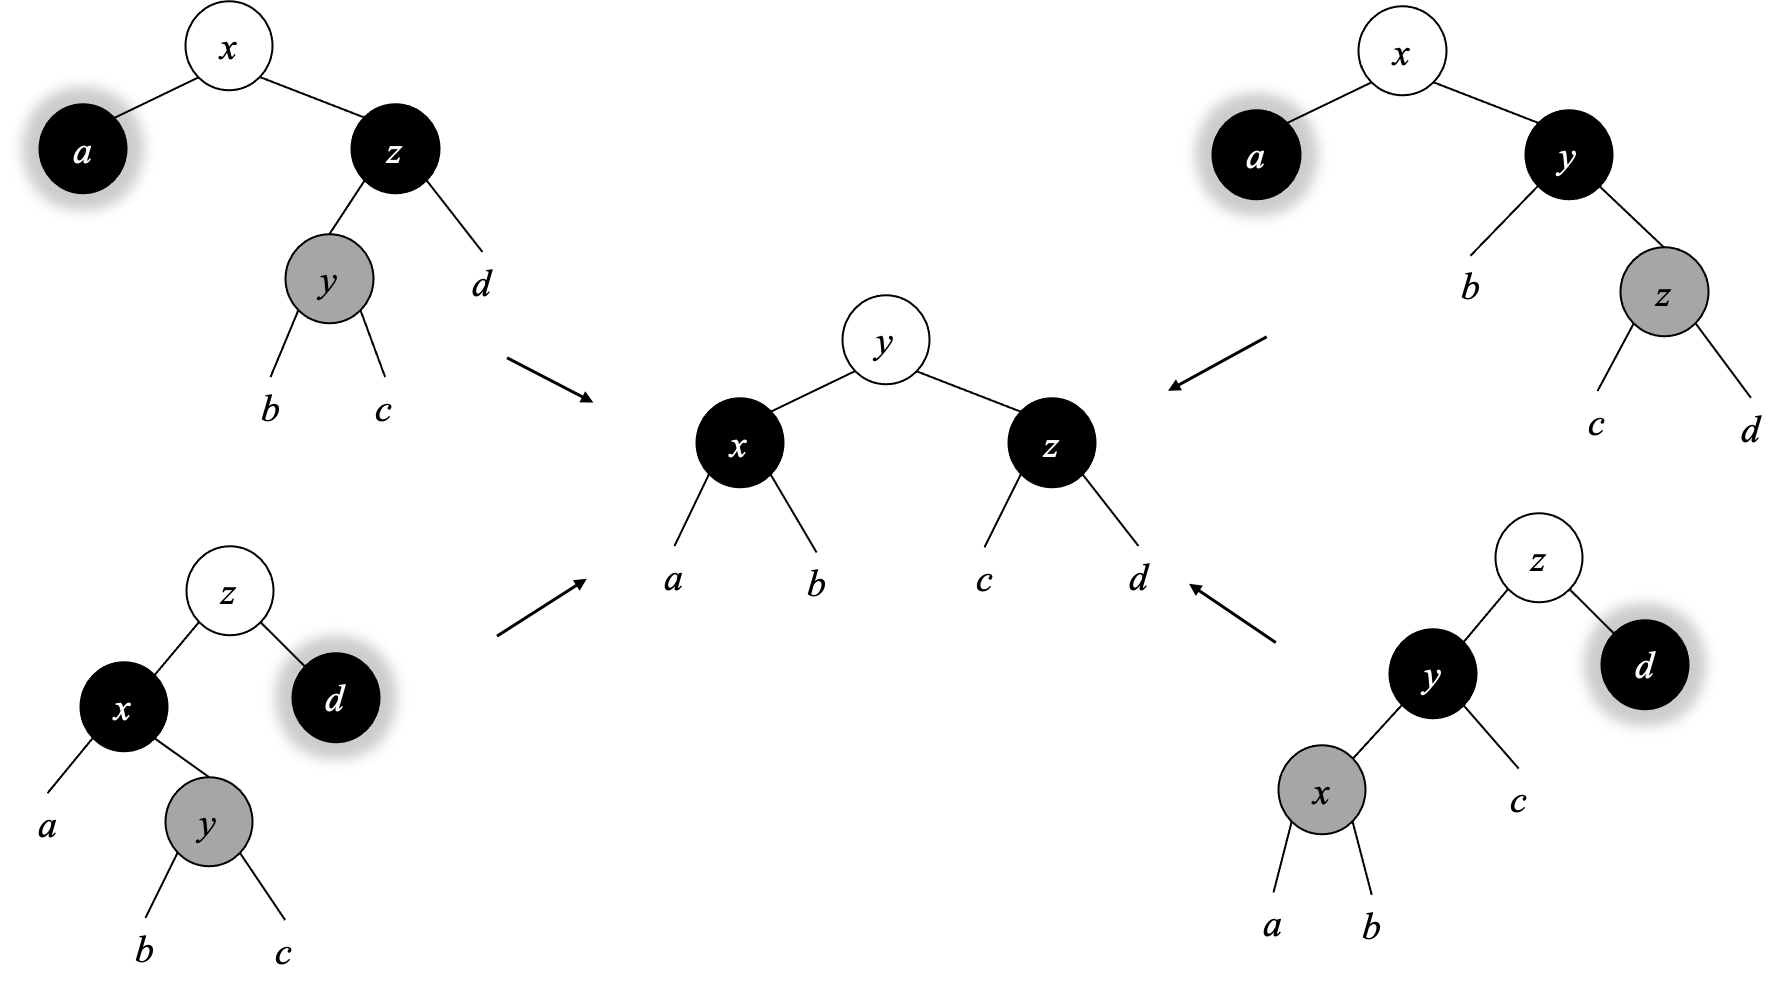
\includegraphics[scale=0.4]{img/del-case1.png}
  \caption{4 sub-cases share the uniformed fixing pattern}
  \label{fig:del-case1}
\end{figure}

The handling of these 4 sub-cases can be realized with pattern matching.

\be
\resizebox{\textwidth}{!}{\ensuremath{
\begin{array}{lcl}
\text{case 1 up left:} & & \\
fixB^2\ \mathcal{C}\ a_{\mathcal{B}^2}\ x\ (\mathcal{B}, (\mathcal{R}, b, y, c), z, d) & = & (\mathcal{C}, (\mathcal{B}, shiftBlack(a_{\mathcal{B}^2}), x, b), y, (\mathcal{B}, c, z, d)) \\
\text{case 1 up right:} & & \\
fixB^2\ \mathcal{C}\ a_{\mathcal{B}^2}\ x\ (\mathcal{B}, b, y, (\mathcal{R}, c, z, d)) & = & (\mathcal{C}, (\mathcal{B}, shiftBlack(a_{\mathcal{B}^2}), x, b), y, (\mathcal{B}, c, z, d)) \\
\text{case 1 bottom left:} & & \\
fixB^2\ \mathcal{C}\ (\mathcal{B}, a, x, (\mathcal{R}, b, y, c))\ z\ d_{\mathcal{B}^2} & = & (\mathcal{C}, (\mathcal{B}, a, x, b), y, (\mathcal{B}, c, z, shiftBlack(d_{\mathcal{B}^2}))) \\
\text{case 1 bottom right:} & & \\
fixB^2\ \mathcal{C}\ (\mathcal{B}, (\mathcal{R}, a, x, b), y, c)\ z\ d_{\mathcal{B}^2} & = & (\mathcal{C}, (\mathcal{B}, a, x, b), y, (\mathcal{B}, c, z, shiftBlack(d_{\mathcal{B}^2}))) \\
\end{array}
}}
\label{eq:db-case-1}
\ee

Where $a_{\mathcal{B}^2}$ means node $a$ is doubly-black, it can be branch or $\pmb{\varnothing}$.

\textbf{Case 2}. {\em The sibling of the doubly-black is red.} We can rotate the tree to turn it into case 1, as shown in figure \ref{fig:del-case2}.

\begin{figure}[htbp]
  \centering
  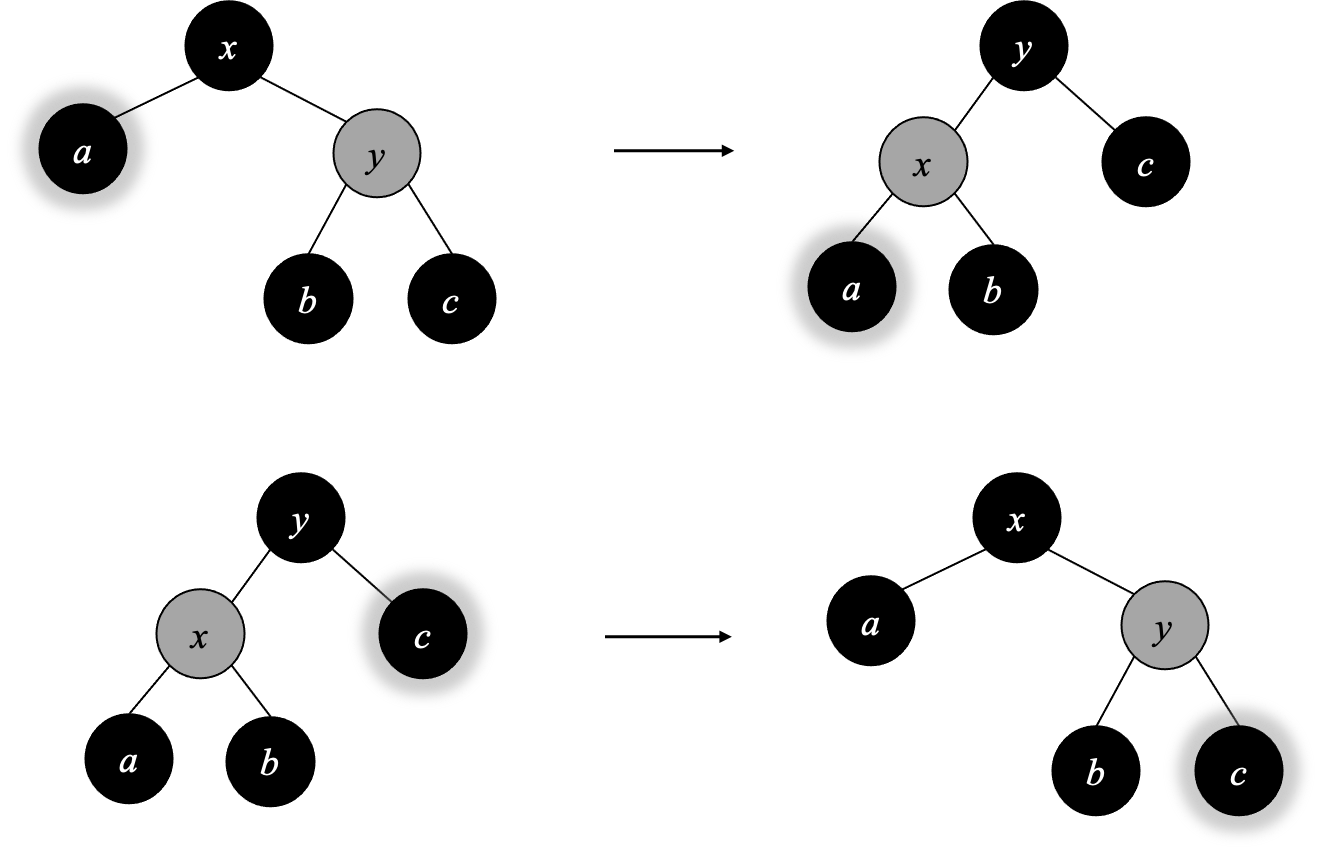
\includegraphics[scale=0.4]{img/del-case2.png}
  \caption{The sibling of the doubly-black is red.}
  \label{fig:del-case2}
\end{figure}

We add this fixing as additional 2 rows in equation (\ref{eq:db-case-1}):

\be
%\resizebox{\textwidth}{!}{\ensuremath{
\begin{array}{lcl}
\text{...} & & \\
\text{case 2 up:} & & \\
fixB^2\ \mathcal{B}\ a_{\mathcal{B}^2}\ x\ (\mathcal{R}, b, y, c) & = & fixB^2\ \mathcal{B}\ (fixB^2\ \mathcal{R}\ a\ x\ b)\ y\ c \\
\text{case 2 bottom:} & & \\
fixB^2\ \mathcal{B}\ (\mathcal{R}, a, x, b)\ y\ c_{\mathcal{B}^2} & = & fixB^2\ \mathcal{B}\ a\ x\ (fixB^2\ \mathcal{R}\ b\ y\ c)
\end{array}
%}}
\label{eq:db-case-2}
\ee

\textbf{Case 3}. {\em The sibling of the doubly-black node, and its two children are all black.} In this case, we can change the color of the sibling node to red; turn the
doubly-black node to black and propagate the doubly-blackness one level
up to the parent node as shown in figure \ref{fig:del-case3}. There are two
symmetric sub-cases.

\begin{figure}[htbp]
  \centering
  \setlength{\unitlength}{1cm}
  \begin{picture}(10, 4)
  \put(5, 2){$\Longrightarrow$}
  \subcaptionbox{Color of $x$ can be either black or red.}{\includegraphics[scale=0.4]{img/case2-a.ps}}
  \subcaptionbox{If $x$ was red, then it becomes black, otherwise, it becomes doubly-black.}{\includegraphics[scale=0.4]{img/case2-a1.ps}}
  \end{picture}
  \\
  \begin{picture}(10, 5)
  \put(5, 2){$\Longrightarrow$}
  \subcaptionbox{Color of $y$ can be either black or red.}{\includegraphics[scale=0.4]{img/case2-b.ps}}
  \subcaptionbox{If $y$ was red, then it becomes black, otherwise, it becomes doubly-black.}{\includegraphics[scale=0.4]{img/case2-b1.ps}}
  \end{picture}
  \\
  \begin{picture}(1, 0.5)\end{picture} %pad
  \caption{propagate the blackness up.} \label{fig:del-case3}
\end{figure}

We go on adding this fixing after formula (\ref{eq:db-case-2}).

\be
fixBlack^2(T) = \left \{
  \begin{array}
  {r@{\quad:\quad}l}
  ... & ... \\
  mkBlk((\mathcal{C}, mkBlk(A), x, (\mathcal{R}, B, y, C))) & p 3.1 \\
  mkBlk((\mathcal{C}, (\mathcal{R}, A, x, B), y, mkBlk(C))) & p 3.2 \\
  ... & ...
  \end{array}
\right .
\label{eq:db-case-3}
\ee

where $p 3.1$ and $p 3.2$ are two patterns as below.

\[
p 3.1 : \left \{ \begin{array}{l}
  T = (\mathcal{C}, A, x, (\mathcal{B}, B, y, C)) \land \\
  color(A) = \mathcal{B}^2 \land color(B) = color(C) = \mathcal{B}
  \end{array} \right \}
\]

\[
p 3.2 : \left \{ \begin{array}{l}
  T = (\mathcal{C}, (\mathcal{B}, A, x, B), y, C) \land \\
  color(C) = \mathcal{B}^2 \land color(A) = color(B) = \mathcal{B}
  \end{array} \right \}
\]

If the doubly black node is doubly black empty node $\Phi$, it can be changed
back to normal empty node after re-coloring. We add the doubly black empty node
handling to (\ref{eq:db-case-3}) as below.

\be
fixBlack^2(T) = \left \{
  \begin{array}
  {r@{\quad:\quad}l}
  ... & ... \\
  mkBlk((\mathcal{C}, mkBlk(A), x, (\mathcal{R}, B, y, C))) & p 2.1 \\
  mkBlk((\mathcal{C}, \phi, x, (\mathcal{R}, B, y, C))) & p 2.1' \\
  mkBlk((\mathcal{C}, (\mathcal{R}, A, x, B), y, mkBlk(C))) & p 2.2 \\
  mkBlk((\mathcal{C}, (\mathcal{R}, A, x, B), y, \phi)) & p 2.2' \\
  ... & ...
  \end{array}
\right .
\label{eq:db-case-3a}
\ee

Where pattern $p 3.1'$ and $p 3.2'$ are defined as the following.

\[
p 3.1' : \left \{ \begin{array}{l}
  T = (\mathcal{C}, \Phi, x, (\mathcal{B}, B, y, C)) \land \\
  color(B) = color(C) = \mathcal{B}
  \end{array} \right \}
\]

\[
p 3.2' : \left \{ \begin{array}{l}
  T = (\mathcal{C}, (\mathcal{B}, A, x, B), y, \Phi) \land \\
  color(A) = color(B) = \mathcal{B}
  \end{array} \right \}
\]

Fixing the doubly-black node with all above different cases is a recursive function.
There are two termination conditions. One contains pattern $p 1.1$ and $p 1.2$,
The doubly-black node was eliminated. The other cases may continuously propagate the
doubly-blackness from bottom to top till the root.
Finally the algorithm marks the root node as black anyway. The doubly-blackness will be
removed.

Put formula (\ref{eq:db-case-1a}), (\ref{eq:db-case-2}), and (\ref{eq:db-case-3a})
together, we can write the final Haskell program.

\begin{lstlisting}
-- the sibling is black, and it has one red child
fixDB color a@(Node BB _ _ _) x (Node B (Node R b y c) z d)
      = Node color (Node B (makeBlack a) x b) y (Node B c z d)
fixDB color BBEmpty x (Node B (Node R b y c) z d)
      = Node color (Node B Empty x b) y (Node B c z d)
fixDB color a@(Node BB _ _ _) x (Node B b y (Node R c z d))
      = Node color (Node B (makeBlack a) x b) y (Node B c z d)
fixDB color BBEmpty x (Node B b y (Node R c z d))
      = Node color (Node B Empty x b) y (Node B c z d)
fixDB color (Node B a x (Node R b y c)) z d@(Node BB _ _ _)
      = Node color (Node B a x b) y (Node B c z (makeBlack d))
fixDB color (Node B a x (Node R b y c)) z BBEmpty
      = Node color (Node B a x b) y (Node B c z Empty)
fixDB color (Node B (Node R a x b) y c) z d@(Node BB _ _ _)
      = Node color (Node B a x b) y (Node B c z (makeBlack d))
fixDB color (Node B (Node R a x b) y c) z BBEmpty
      = Node color (Node B a x b) y (Node B c z Empty)
-- the sibling is red
fixDB B a@(Node BB _ _ _) x (Node R b y c) = fixDB B (fixDB R a x b) y c
fixDB B a@BBEmpty x (Node R b y c) = fixDB B (fixDB R a x b) y c
fixDB B (Node R a x b) y c@(Node BB _ _ _) = fixDB B a x (fixDB R b y c)
fixDB B (Node R a x b) y c@BBEmpty = fixDB B a x (fixDB R b y c)
-- the sibling and its 2 children are all black, propagate the blackness up
fixDB color a@(Node BB _ _ _) x (Node B b y c) = makeBlack (Node color (makeBlack a) x (Node R b y c))
fixDB color BBEmpty x (Node B b y c) = makeBlack (Node color Empty x (Node R b y c))
fixDB color (Node B a x b) y c@(Node BB _ _ _) = makeBlack (Node color (Node R a x b) y (makeBlack c))
fixDB color (Node B a x b) y BBEmpty = makeBlack (Node color (Node R a x b) y Empty)
-- otherwise
fixDB color l k r = Node color l k r
\end{lstlisting}

The deletion algorithm takes $O(\lg n)$ time to delete a key from
a red-black tree with $n$ nodes.

\begin{Exercise}

\begin{itemize}
\item As we mentioned in this section, deletion can be implemented
by just marking the node as deleted without actually removing it.
Once the number of marked nodes exceeds 50\%, a tree re-build is performed. Try to implement this
method in your favorite programming language.
\item Why needn't enclose $mkBlk$ with a call to $fixBlack^2$ explicitly in the definition of $del(T, k)$?
\end{itemize}

\end{Exercise}

\section{Imperative red-black tree algorithm $\star$}
\index{red-black tree!imperative insertion}

We almost finished all the content in this chapter. By induction
the patterns, we can implement the red-black tree in a simple way
compare to the imperative tree rotation solution. However, we
should show the comparator for completeness.

For insertion, the basic idea is to use the similar algorithm
as described in binary search tree. And then fix the balance
problem by rotation and return the final result.

\begin{algorithmic}[1]
\Function{Insert}{$T, k$}
  \State $root \gets T$
  \State $x \gets$ \Call{Create-Leaf}{$k$}
  \State \Call{Color}{$x$} $\gets$ RED
  \State $p \gets$ NIL
  \While{$T \neq$ NIL}
    \State $p \gets T$
    \If{$k <$ \Call{Key}{$T$}}
      \State $T \gets $ \Call{Left}{$T$}
    \Else
      \State $T \gets $ \Call{Right}{$T$}
    \EndIf
  \EndWhile
  \State \Call{Parent}{$x$} $\gets p$
  \If{$p =$ NIL} \Comment{tree $T$ is empty}
    \State \Return $x$
  \ElsIf{$k <$ \Call{Key}{$p$}}
    \State \Call{Left}{$p$} $\gets x$
  \Else
    \State \Call{Right}{$p$} $\gets x$
  \EndIf
  \State \Return \Call{Insert-Fix}{$root, x$}
\EndFunction
\end{algorithmic}

The only difference from the binary search tree insertion algorithm
is that we set the color of the new node as red, and perform fixing
before return. Below is the example Python program.

\lstset{language=Python}
\begin{lstlisting}
def rb_insert(t, key):
    root = t
    x = Node(key)
    parent = None
    while(t):
        parent = t
        if(key < t.key):
            t = t.left
        else:
            t = t.right
    if parent is None: #tree is empty
        root = x
    elif key < parent.key:
        parent.set_left(x)
    else:
        parent.set_right(x)
    return rb_insert_fix(root, x)
\end{lstlisting}

There are 3 base cases for fixing, and if we take the left-right
symmetric into consideration. there are total 6 cases.
Among them two cases can be merged together, because they all have
uncle node in red color, we can toggle the parent color and
uncle color to black and set grand parent color to red.
With this merging, the fixing algorithm can be realized as the following.

\begin{algorithmic}[1]
\Function{Insert-Fix}{$T, x$}
  \While{\Call{Parent}{$x$} $\neq$ NIL $\land$ \textproc{Color}(\Call{Parent}{$x$}) = RED}
    \If{\textproc{Color}(\Call{Uncle}{$x$}) $=$ RED}
      \Comment{Case 1, x's uncle is red}
      \State \textproc{Color}(\Call{Parent}{$x$}) $\gets$ BLACK
      \State \textproc{Color}(\Call{Grand-Parent}{$x$}) $\gets$ RED
      \State \textproc{Color}(\Call{Uncle}{$x$}) $\gets$ BLACK
      \State $x \gets$ \Call{Grand-Parent}{$x$}
    \Else
      \Comment{x's uncle is black}
      \If{\Call{Parent}{$x$} = \textproc{Left}(\Call{Grand-Parent}{$x$})}
        \If{ $x =$ \textproc{Right}(\Call{Parent}{$x$})}
          \Comment{Case 2, x is a right child}
          \State $x \gets$ \Call{Parent}{$x$}
          \State $T \gets$ \Call{Left-Rotate}{$T, x$}
        \EndIf
        \Comment{Case 3, x is a left child}
        \State \textproc{Color}(\Call{Parent}{$x$}) $\gets$ BLACK
        \State \textproc{Color}(\Call{Grand-Parent}{$x$}) $\gets$ RED
        \State $T \gets$ \textproc{Right-Rotate}($T$, \Call{Grand-Parent}{$x$})
      \Else
         \If{ $x =$ \textproc{Left}(\Call{Parent}{$x$})}
          \Comment{Case 2, Symmetric}
          \State $x \gets$ \Call{Parent}{$x$}
          \State $T \gets$ \Call{Right-Rotate}{$T, x$}
        \EndIf
        \Comment{Case 3, Symmetric}
        \State \textproc{Color}(\Call{Parent}{$x$}) $\gets$ BLACK
        \State \textproc{Color}(\Call{Grand-Parent}{$x$}) $\gets$ RED
        \State $T \gets$ \textproc{Left-Rotate}($T$, \Call{Grand-Parent}{$x$})
      \EndIf
    \EndIf
  \EndWhile
  \State \Call{Color}{$T$} $\gets$ BLACK
  \State \Return $T$
\EndFunction
\end{algorithmic}

This program takes $O(\lg n)$ time to insert a new key to the red-black tree.
Compare this pseudo code and the $balance$ function we defined in previous
section, we can see the difference. They differ not only in terms of
simplicity, but also in logic. Even if we feed the same series of keys to
the two algorithms, they may build different red-black trees. There
is a bit performance overhead in the pattern matching algorithm.
Okasaki discussed about the difference in detail in his paper\cite{okasaki}.

Translate the above algorithm to Python yields the below program.

\begin{lstlisting}
# Fix the red->red violation
def rb_insert_fix(t, x):
    while(x.parent and x.parent.color==RED):
        if x.uncle().color == RED:
            #case 1: ((a:R x:R b) y:B c:R) ==> ((a:R x:B b) y:R c:B)
            set_color([x.parent, x.grandparent(), x.uncle()],
                      [BLACK, RED, BLACK])
            x = x.grandparent()
        else:
            if x.parent == x.grandparent().left:
                if x == x.parent.right:
                    #case 2: ((a x:R b:R) y:B c) ==> case 3
                    x = x.parent
                    t=left_rotate(t, x)
                # case 3: ((a:R x:R b) y:B c) ==> (a:R x:B (b y:R c))
                set_color([x.parent, x.grandparent()], [BLACK, RED])
                t=right_rotate(t, x.grandparent())
            else:
                if x == x.parent.left:
                    #case 2': (a x:B (b:R y:R c)) ==> case 3'
                    x = x.parent
                    t = right_rotate(t, x)
                # case 3': (a x:B (b y:R c:R)) ==> ((a x:R b) y:B c:R)
                set_color([x.parent, x.grandparent()], [BLACK, RED])
                t=left_rotate(t, x.grandparent())
    t.color = BLACK
    return t
\end{lstlisting}

Figure \ref{fig:imperative-insert} shows the results of feeding same
series of keys to the above python insertion program. Compare them with
figure \ref{fig:insert-example}, one can tell the difference clearly.

\begin{figure}[htbp]
   \centering
   \subcaptionbox{}{\includegraphics[scale=0.4]{img/clrs-fig-13-4.ps}}
   \subcaptionbox{}{\includegraphics[scale=0.4]{img/python-insert.ps}}
   \caption{Red-black trees created by imperative algorithm.}
   \label{fig:imperative-insert}
\end{figure}

We put the red-black tree delete algorithm in imperative settings in Appendix B,
because it is more complex than the insertion.

\section{More words}
Red-black tree is the most popular implementation of balanced binary search
tree. Another one is the AVL tree, which we'll introduce in next chapter.
Red-black tree can be a good start point for more data structures. If we
extend the number of children from 2 to $k$, and keep the balance as well,
it leads to B-tree, If we store the data along with edge but not inside
node, it leads to Tries. However, the multiple cases handling and the long
program tends to make new comers think red-black tree is complex.

Okasaki's work helps making the red-black tree much easily understand.
There are many implementation in other programming languages in that
manner \cite{rosetta}. It's also inspired me to find the pattern matching
solution for Splay tree and AVL tree etc.

\section{Appendix: Example programs}

Definition of red-black tree node with parent field. When not explicitly defined, the color of the new node is red by default.

\begin{lstlisting}[language = Bourbaki]
data Node<T> {
    T key
    Color color
    Node<T> left
    Node<T> right
    Node<T> parent

    Node(T x) = Node(null, x, null, Color.RED)

    Node(Node<T> l, T k, Node<T> r, Color c) {
        left = l, key = k, right = r, color = c
        if (left != null) then left.parent = this
        if (right != null) then right.parent = this
    }
}
\end{lstlisting}

\begin{thebibliography}{99}

\bibitem{CLRS}
Thomas H. Cormen, Charles E. Leiserson, Ronald L. Rivest and Clifford Stein.
``Introduction to Algorithms, Second Edition''. ISBN:0262032937. The MIT Press. 2001

\bibitem{okasaki}
Chris Okasaki. ``FUNCTIONAL PEARLS Red-Black Trees in a Functional Setting''. J. Functional Programming. 1998

\bibitem{okasaki-blog}
Chris Okasaki. ``Ten Years of Purely Functional Data Structures''. http://okasaki.blogspot.com/2008/02/ten-years-of-purely-functional-data.html

\bibitem{wiki-rbt}
Wikipedia. ``Red-black tree''. \url{http://en.wikipedia.org/wiki/Red-black\_tree}

\bibitem{rosetta}
Pattern matching. \url{http://rosettacode.org/wiki/Pattern\_matching}

\end{thebibliography}

\ifx\wholebook\relax\else
\end{document}
\fi
